\documentclass[12pt, a4paper]{article}

\usepackage[utf8]{inputenc}
\usepackage{amsmath}
\usepackage{amssymb}
\usepackage{physics}
\usepackage{pgfplots}
\usepackage{mathtools}
\usepackage[hmarginratio=1:1]{geometry}
\usepackage{float}
\usepackage[affil-it]{authblk}
\usepackage{graphicx}
% \usepackage{wrapfig}
\usepackage{subfig}
\graphicspath{ {./res/} }

% \usepackage{xcolor}
% \pagecolor[rgb]{0,0,0}
% \color[rgb]{0.5,0.5,0.5}

\title{Modelling the oscillation of walking humans}
\author{Martin Velikov}
\date{August 2022}

\begin{document}

% title & contents
\maketitle
\tableofcontents

\pagebreak
% content
\section{Introduction}
\subsection{Background}
Walking is one of the things that we do most as humans. It is the most
fundamental way of transportation, serving us faithfully for roughly 6 million
years. As one of the few bipedal mammals on the Earth, our motion during walking
is complex and rather effective for the energy we expend doing it. We have tried
to analyze the way we walk, in order to create better tools that, well, enable
us to walk better, like shoes or corrective soles. One fundamental side product
of our peculiar way of motion is that the entire upper body undergoes vertical
oscillation , or put simply, we move and sway up and down whenever we walk.

\subsection{Aim}
The aim of this investigation is, using mathematical functions, to model this
vertical oscillation of the human body while walking.

\subsection{Applications}
There are numerous applications of modern technology where being able to model
the oscillation from walking is invaluable. For example, optical image
stabilization present in nearly all modern video cameras aims to minimize the
'screen shake' by compensating with movement in the lens of the camera. A model
of oscillation while walking could aid this endeavor by allowing more
predictable corrections to be made by software, which would benefit us in
several areas such as film entertainment and physiological analysis.
Additionally, motion discomfort has been a key barrier into the widespread
adoption of virtual reality into our daily lives. Some people do not feel
comfortable in an environment disconnected from their physical presence, and
being able to model a person's sway while walking could aid the endeavor to
smooth, or even recreate it in a virtual world, therefore alleviating this
discomfort and opening the possibilities for a more broad adoption of VR
technology.

\subsection{Personal motivation}
todo

\section{Data collection}
\subsection{Background}
In order to model the vertical oscillation of human walking, it must first be
measured accurately. I considered several possibilities for how I can achieve
this, including making a kinematic model of a human leg, or simply filming a
person walking and then tracing over the footage to obtain the path of the leg.
However, both methods posed significant issues with them:
\begin{itemize}
    \item The kinematic model may not be perfectly applicable to the shape,
          proportion \& movement range of a real human leg. It would be very
          complex to make it even approximate the properties of a real human
          leg, which would not be worthwhile since I would only be trying to
          extract data from it once or twice.
    \item Tracing over a film of someone walking poses several accuracy \&
          precision errors. For example, determining the location of the part of
          the leg that needs to be tracked would rely on a visual estimate,
          which is subject to the many issues of a video camera, such as
          parallax error (as an orthographic camera cannot physically exist),
          motion blur, resolution \& lens distortion.
\end{itemize}

\subsection{Solution}
In order to address the issues with the initially proposed data collection
methods, I opted for a more robust \& accurate to real life measurment technique
of actually motion tracking in 3D while walking. For the purposes of this
investigation, I did not require full limb-for-limb tracking - only my head, and
the bases of my feet. \\

For the task, I used an Oculus Rift virtual reality headset and motion
controller pair in an improvised setup. Although the controllers are meant to be
used for hand tracking, I fixed them securely to my ankles, as close as possible
to my heel, and found that they still tracked the motion of walking accurately.
\\

For the software, after some research on what popular dance groups such and
other "fully virtual dancers" use, I found that they all used the same set of
software, albeit with a more elaborate setup than my improvised one.

\begin{figure}[H]
    \centering
    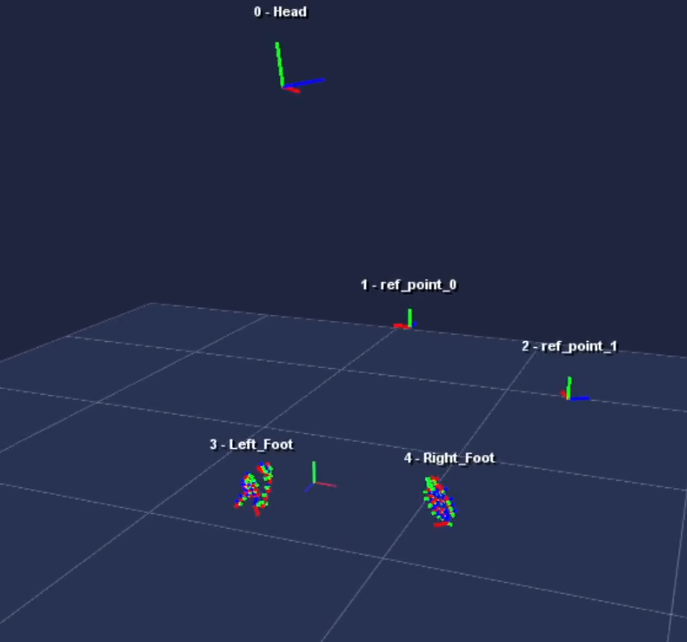
\includegraphics[width=10cm]{mocap_software}
    \caption{Motion tracking setup with person in the middle of a step}
    \label{mocap}
\end{figure}

Figure \ref{mocap} shows the computer side of the tracking setup. I used two IR
tracking sensors (\texttt{ref\_point\_0} and \texttt{ref\_point\_1}) pointed at
the area I was to walk through, and set up the software so that it tracked my
head and feet, to which the tracking points were attached to. \\

After some testing with moving the tracking point along a ruler, I found that
the position data returned was accurate to two millimeters, which is far beyond
anything that would have been achieved with the two initially proposed data
collection methods.

\subsection{Results}

\begin{figure}[H]
    \centering
    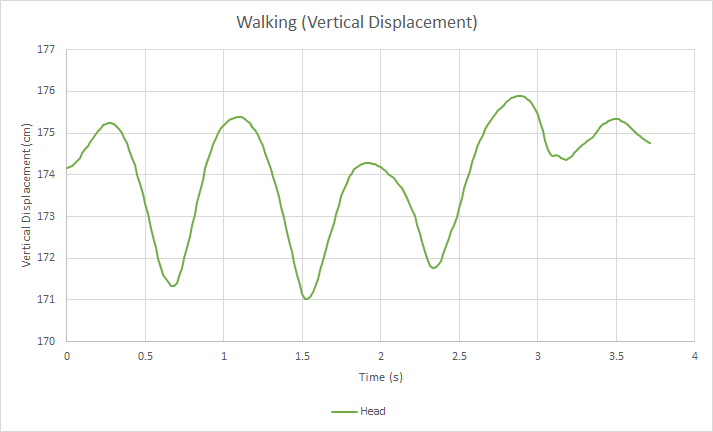
\includegraphics[width=10cm]{head_vert.png}
    \caption{Vertical motion of head}
    \label{head_y}
\end{figure}

Figure \ref{head_y} depicts the vertical displacement of my head from the floor.
It can be observed that it resembles some sort of wave with crests \& troughs,
which makes sense - a person walking would go up and down periodically with
every step. From the graph, it is evident that the 4 steps were taken, indicated
by the 4 crests. It is also noteworthy that the troughs are far sharper than the
crests, which may be a product of the foot of the walker hitting the floor (the
trough), and the leg moving through the air (the crest). Anyhow, this
interesting pattern warrants investigation, as the head is the best indicator of
the general vertical motion of the body in this case.

\begin{figure}[H]
    \centering
    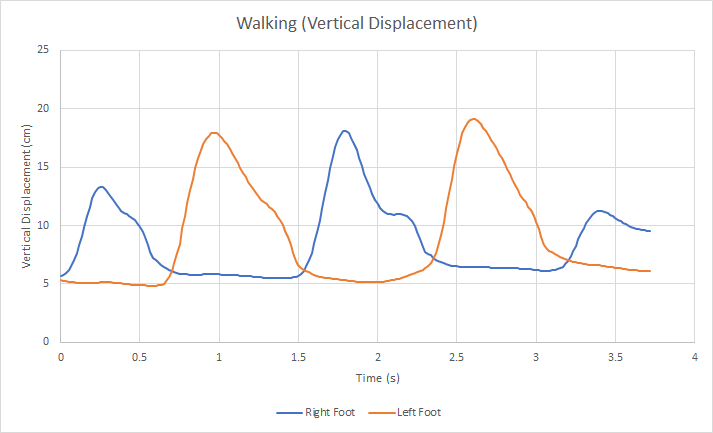
\includegraphics[width=10cm]{feet_vert.png}
    \caption{Vertical motion of feet over time}
    \label{feet_y}
\end{figure}

Figure \ref{feet_y} depicts the motion of my feet vertically. It is evident from
this that each foot has two crests, for a total of four steps, which matches up
nicely with the observations made from Figure \ref{head_y}. The shape of these
crests and troughs is peculiar, but anyhow seem to follow an explicable pattern.
It seems like the graphs of the right and left foot are completely out of phase,
which makes sense given that only one foot can be on the ground at a time,
during which the other one must be in the process of taking a step. \\

The shape of the troughs makes sense as well, as they are almost perfectly flat.
The small amount of curvature that precedes the large peak is most likely caused
by the heel being lifted in the air as the foot is getting ready for another
step. This is further supported by the fact that at the beginning, the left
foot's first trough is far sharper than the succeeding ones, because one leg of
the person walking would be starting the step from a standstill. \\

It is also noteworthy to talk about the small secondary bump following the
crest, visible in all crests, but most prominent in the second step of the right
foot. This could be explained as the foot of the person walking maintaining an
approximate level height, then suddenly returning back to the ground on the
"falling edge" of a step. In reality, the prominence of this secondary bump
could be specific to the walking style of the person, however, it is significant
enough to the point where it cannot be disregarded as simple error.

\begin{figure}[H]
    \centering
    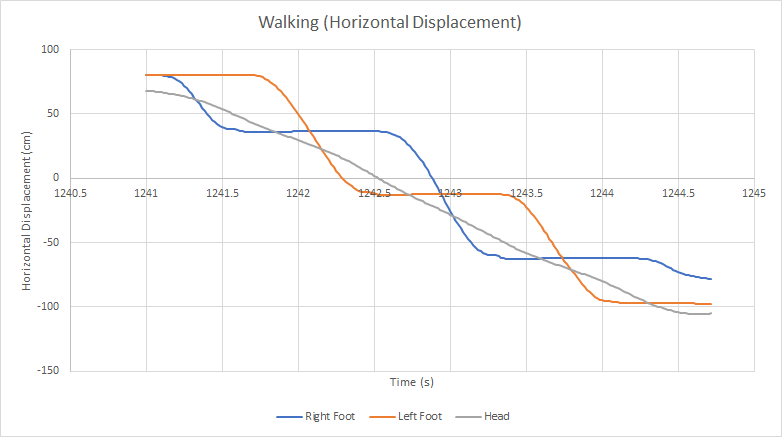
\includegraphics[width=11cm]{motion_horiz.png}
    \caption{Horizontal motion of ankles and head}
    \label{horiz}
\end{figure}

Figure \ref{horiz} shows the horizontal motion of the three tracked points
throughout the walk. Its data is not necessarily relevant to modelling the
vertical oscillation, however it is able to provide some key insights into the
motion of the person during the walk. It is evident that generally, for all
three graphs, the motion happens in one direction, which is forward, or, on the
graph, towards $-\infty$. The graphs of horizontal motion of the feet alternate
in successive "dips", which resemble one step, where one foot is stationary
while the other is free to move forward. The graph of the motion of the head is
very close to being linear, and it appears to pass through the graphs of both
feet. In the regions where the graph of a foot is above the graph of the head,
it would be lagging behind in real life, while being below would mean it is
ahead. Generally, it can be observed that the regions where it is found above
the graph of the head (lagging behind) are greater than the regions where it is
behind, which coincides with the data for the vertical motion of the feet, where
the falling edge of each crest is generally longer than its rising edge.

\section{Modelling options}
In terms of modelling the curves, a polynomial may prove to provide the most
precise model of the dataset, especially for the more peculiar graphs like those
of the motion of the feet. There are three main advantage of using polynomials
to model these motions. First, polynomials are inexpensive to compute and work
with, since they only use multiplication and addition, something both humans and
computers are quite adept at. This makes representing something as a polynomial
very worthwhile. Based off of this, the second advantage - fitting polynomials
to best approximate data is a well-explored topic, with several well-established
working methods which can be used to provide shockingly accurate results. The
last of these advantages is specific to the shape of our graph - it has smooth
curves, which polynomials are really good at representing. \\

There are several relatively easy methods to fit polynomials to a function,
supposing that you can find its derivative. One possible method is constructing
a Taylor polynomial, which would be accurate around the point which is
constructed. Unfortunately, for our case, we are trying to fit through a dataset
of points, for which finding the derivative (or more importantly, higher-order
derivatives) might prove challenging without, paradoxically, knowing how to
define the original function. \\

Ultimately, the method that is most applicable to this type of task is some type
of regression. Since we are trying to fit a polynomial to the data, polynomial
regression with some cost function will work nicely. For the cost function, the
"least squares" has been chosen for its simplicity, effectivity and widespread
use. \\

\section{Least squares polynomial fitting}
\subsection{Theory}
Suppose that there is a polynomial $P$ of degree $k$ so that
\begin{align*}
    P(x)= a_0 + a_1 x + \cdots + a_{k-1} x^{k-1} + a_k x^k
\end{align*}

The coefficients $a_0$ through $a_k$ are the unknowns that must be solved for,
defining the shape of the polynomial. Assuming one wants to fit this polynomial
to a set of points, it would be useful to know how accurately it can model the
dataset, given a guess of the its coefficients $a_0 \cdots a_k$.

\begin{figure}[H]
    \centering
    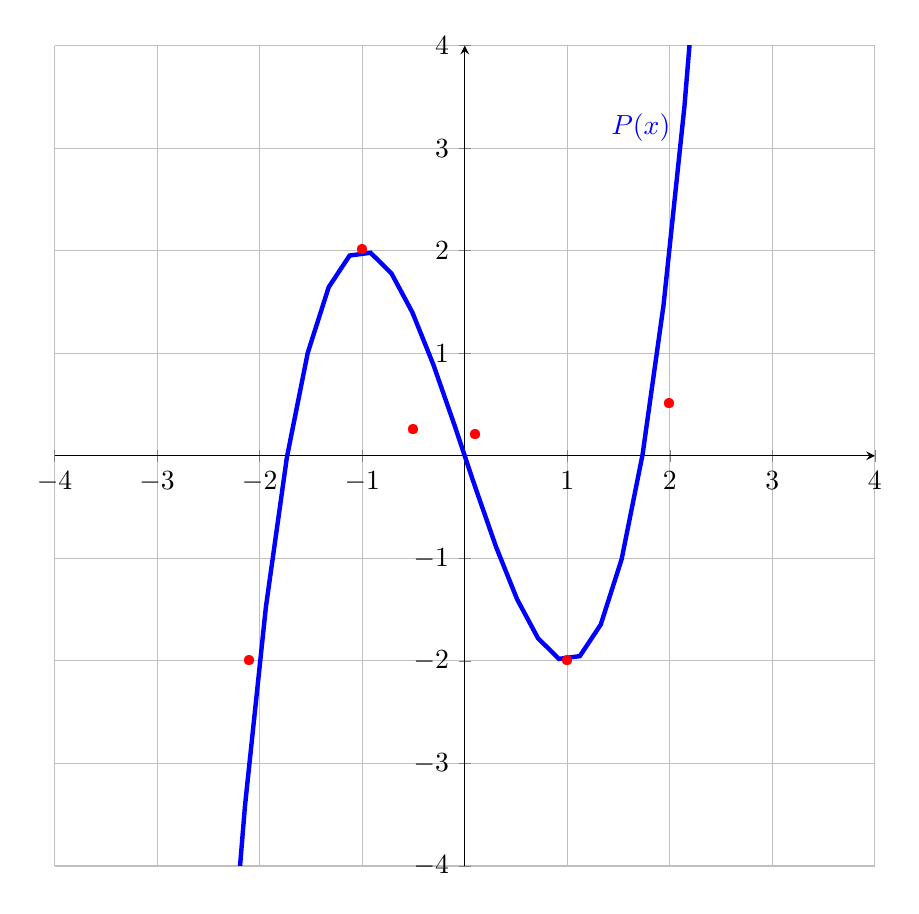
\begin{tikzpicture}
        \begin{axis}[
                axis y line=center,
                axis x line=middle,
                xmin=-4,
                xmax=4,
                ymin=-4,
                ymax=4,
                height=12.0cm,
                width=12.0cm,
                grid,
                xtick={-4,...,4},
                ytick={-4,...,4},
            ]
            \addplot [domain=-5:5, samples=50, mark=none, ultra thick, blue] {x^3-3*x};
            \node [left, blue] at (axis cs: 2.1, 3.2) {$P(x)$};
            \node [red] at (axis cs: 1, -2) {\textbullet};
            \node [red] at (axis cs: 2, 0.5) {\textbullet};
            \node [red] at (axis cs: -0.5, 0.25) {\textbullet};
            \node [red] at (axis cs: -2.1, -2) {\textbullet};
            \node [red] at (axis cs: 0.1, 0.2) {\textbullet};
            \node [red] at (axis cs: -1, 2) {\textbullet};
        \end{axis}
    \end{tikzpicture}
    \caption{
        Example cubic ($k=3$) $P(x)$ fitting 5 points.
    }
    \label{fig1}
\end{figure}

Figure \ref{fig1} depicts one such cubic polynomial. It is evident from the
graph that $P(x)$ does not exactly pass through every point - rather, there is a
slight difference for every point it passes by. Let one of these points be
represented as $(x, y)$. The vertical difference $r$ between this point and the
graph of $P$ could be simply represented by

\begin{align*}
    r=|y-P(x)|
\end{align*}

The absolute value of the difference is used, as $r$ should be indicative of the
deviation from the graph, the direction of difference is irrelevant.
Additionally, instead  of taking its modulus, it can simply be squared in order
to accentuate any error, and be wieldy to derive.  This leaves the final
equation of the difference $r$ between a point $(x, y)$ as

\begin{align*}
    r=(y-P(x))^2
\end{align*}

The total measure of deviation $R^2$ from the graph $P(x)$, called the
"residual", can be obtained by summing up the aforementioned vertical
differences for $n$ points with coordinates $(x, y)$:

\begin{align*}
    R^2 & = \sum^n_{i=1}[y_i-P(x_i)]^2 \\
    % &= \sum^n_{i=1}[
    %     y_i - (a_0 + a_1 x_i + \cdots + a_{k-1} x_i^{k-1} + a_k x_i^k)]^2
\end{align*}

The partial derivative of the residual with respect to each coefficient can be
found, and set to zero in order to ensure that coefficient contributes a minimum
of the error in terms of the entire equation - this effectively minimizes $R^2$,
which is the goal of this method. This results in the following system of
equations:

\begin{align*}
    \frac{\partial (R^2)}{\partial a_0}     & = -2 \sum^n_{i=1}[y_i-P(x_i)] x^0     & = 0 \\
    \frac{\partial (R^2)}{\partial a_1}     & = -2 \sum^n_{i=1}[y_i-P(x_i)] x^1     & = 0 \\
                                            & \vdotswithin{=}                             \\
    \frac{\partial (R^2)}{\partial a_{k-1}} & = -2 \sum^n_{i=1}[y_i-P(x_i)] x^{k-1} & = 0 \\
    \frac{\partial (R^2)}{\partial a_k}     & = -2 \sum^n_{i=1}[y_i-P(x_i)] x^k     & = 0
\end{align*}

From this point, the method requires solving the above system for the most
closely fitting coefficients, ie. minimizing $R^2$. There are several methods
through which this system of equations can be simplified and solved, the proof
of which, however, is beyond the scope of this investigation. After
simplification, the matrix system can be represented as

\begin{align*}
    \begin{bmatrix}
        1      & x_1     & x_1^2     & \cdots & x_1^{k-1}     & x_1^k     \\
        1      & x_2     & x_2^2     & \cdots & x_2^{k-1}     & x_2^k     \\
        \vdots & \vdots  & \vdots    & \ddots & \vdots        & \vdots    \\
        1      & x_{n-1} & x_{n-1}^2 & \cdots & x_{n-1}^{k-1} & x_{n-1}^k \\
        1      & x_n     & x_n^2     & \cdots & x_n^{k-1}     & x_n^k
    \end{bmatrix}
    \begin{bmatrix}
        a_1 \\ a_2 \\ \vdots \\ a_{k-1} \\ a_k
    \end{bmatrix}
    =
    \begin{bmatrix}
        y_1 \\ y_2 \\ \vdots \\ y_{n-1} \\ y_n
    \end{bmatrix}
\end{align*}

An interesting point about this method is that if the number of points $n$ that
the polynomial must be fit to exceeds the degree $k$, the polynomial can never
pass through all of them exactly, which makes sense given that the polynomial
may only have a maximum of $k-1$ turning points. This means that the above
system of matrices is "over-determined", that is, it can never give a perfect
solution in terms of coefficients, only the closest approximation. \\

As for solving the system, multiplying by the transpose $X^T$ of the matrix with
x-terms $X$ would yield a square linear system which can then be solved
numerically for the coefficients in the vector $\vec{a}$.

\begin{align*}
    X^TX\vec{a}=X^T\vec{y}
\end{align*}

As mentioned above, and in the case that applies to solving this problem, a
well-formed solution to this system does not exist most of the time. However, if
the degree $k$ is greater than $n$, the system can be solved for a single vector
of solutions by simply inverting $X^TX$:

\begin{align*}
    \vec{a}=(X^TX)^{-1}X^T\vec{y}
\end{align*}

\subsection{Application \& Exploration}
Now that the underlying method that powers this type of polynomial regression is
known, it is possible to apply it to the dataset. While a polynomial might
accurately model one crest or trough of a step, in reality it would not be
practical to model the entire collected data-set with just one. There are
several ways to account for these issues. \\

\subsubsection{Even "naive" segmentation}
\label{section_naive_seg}
A naive solution to this problem is to segment the entire domain into even
chunks, then fit a polynomial to the portion of the graph (drawn as a punctured
line) in those sub-regions (divided vertically with dotted lines):

\begin{figure}[H]
    \centering
    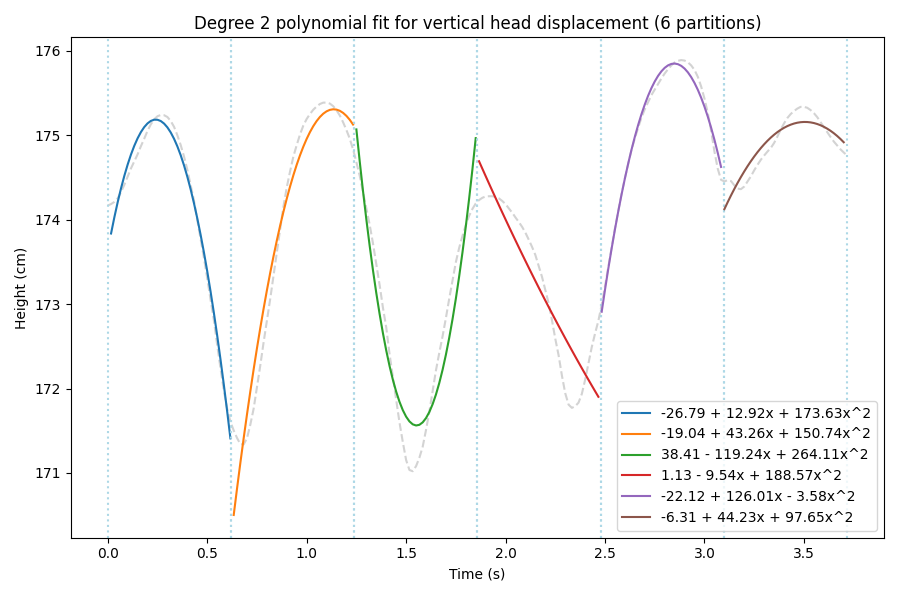
\includegraphics[width=12cm]{p_naive_head_2.png}
    \caption{Naive quadratic fitting for vertical head oscillation data}
    \label{naive_head}
\end{figure}

\begin{figure}[H]
    \centering
    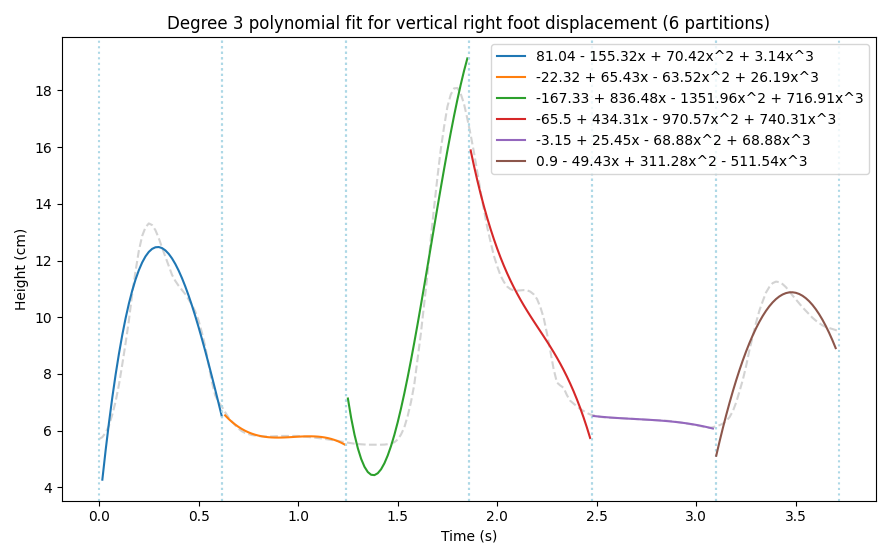
\includegraphics[width=12cm]{p_naive_right_3.png}
    \caption{Naive cubic fitting for vertical right foot oscillation data}
    \label{naive_right}
\end{figure}

There are several main observations that can be made from these naive fitting
attempts: first, from Figure \ref{naive_head}, it is evident that all crests and
troughs are smooth and symmetrical enough so that a quadratic can accurately
model them. This should be kept in mind as it will become important when trying
to refine the fitting method. While the first crest in Figure \ref{naive_head}
appears to be well-fitted, the same cannot be said for the succeeding crests or
troughs.

A possible explanation for this is that the selection of sub-regions does not
respect any of the graph features that a quadratic might benefit from, like the
aforementioned smooth curvature at the crests and troughs. For example, the
third crest's equation (red) is a quadratic that acts very similarly to a linear
in the region it is meant to approximate, since there are not enough turning
points for it to assume the necessary shape. The result of this, as we can see,
is not a very good fit.

In the more complex graph of Figure \ref{naive_right}, this is further
reciprocated. Even though a higher degree of polynomial is used, some regions of
the graph are fitted far better than others, like the first crest compared to
the second, which, due to the naive segmentation, is forcefully cut in two also
resulting in a poor fit.

\subsubsection{Peak segmentation}
In order to address the issues found in \ref{section_naive_seg}, and take
advantage of the patterns identified, we are going to have to examine our
dataset more closely. Polynomial functions are able to fit a dataset
much more closely if the area over which they are fitted is of a similar shape
to them. For example, curved crests and troughs are present in the dataset here,
and they can almost perfectly be fit by a quadratic.

\begin{figure}[H]
    \centering
    \subfloat[\centering Example of a quadratic that fits the crest well]{
        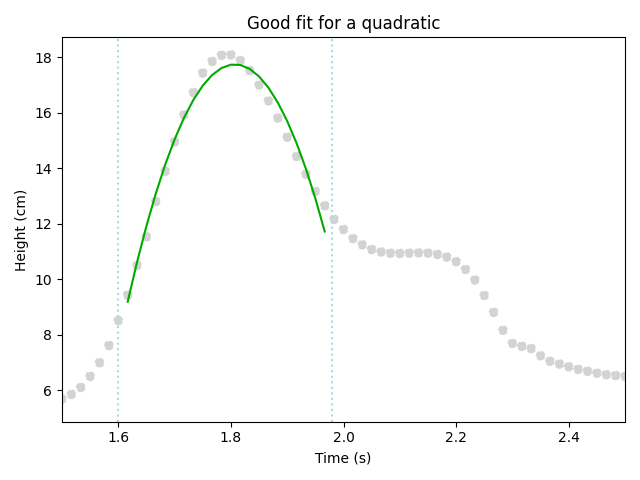
\includegraphics[width=0.5\textwidth]{good_fit.png}
        \label{good_quadratic}
    }
    \subfloat[\centering Example of a quadratic with a poor fit]{
        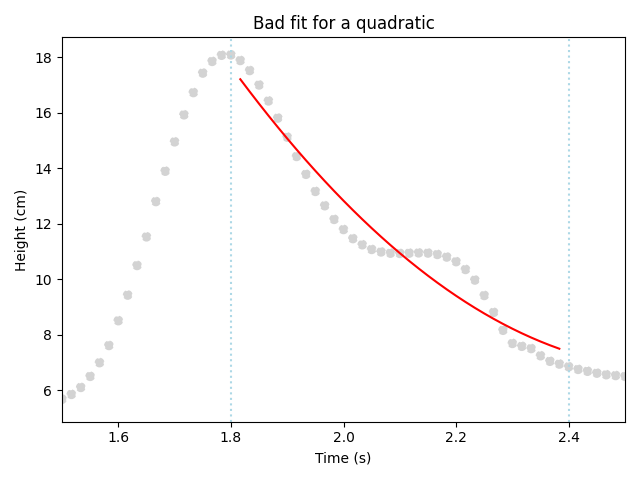
\includegraphics[width=0.5\textwidth]{bad_fit.png}
        \label{bad_quadratic}
    } 
    \caption{ Examples of how the region over which a polynomial is fit can
    drastically affect the accuracy of the fit }
    \label{bad_good_quadratics}
\end{figure}

In Figure \ref{good_quadratic}, the crest can be pefectly fit by a concave down
quadratic, as the region in which the regression was performed was limited to
just around the crest. In contrast, Figure \ref{bad_quadratic} shows a misplaced
quadratic that is trying to fit an area not suited for its shape, resulting in
heavy deviations from the data. \\

Knowing this, it is possible to improve the segmentation method to look for
areas that might be a good fit for specific polynomial functions. For a
quadratic, looking for the crests and troughs to harness the aforementioned
benefits from their shape is a good staring point. \\ 

Crests and troughs can be considered the local minima and maxima of the data at
that point. It is a property of functions that these minimum and maximum points
are also turning points, meaning the derivative of the function changes sign
around them. Applying this to the current data, it is sufficient to find a point
around which both neighbouring points are either both above or both below in the
y-axis.

\begin{figure}[H]
    \centering
    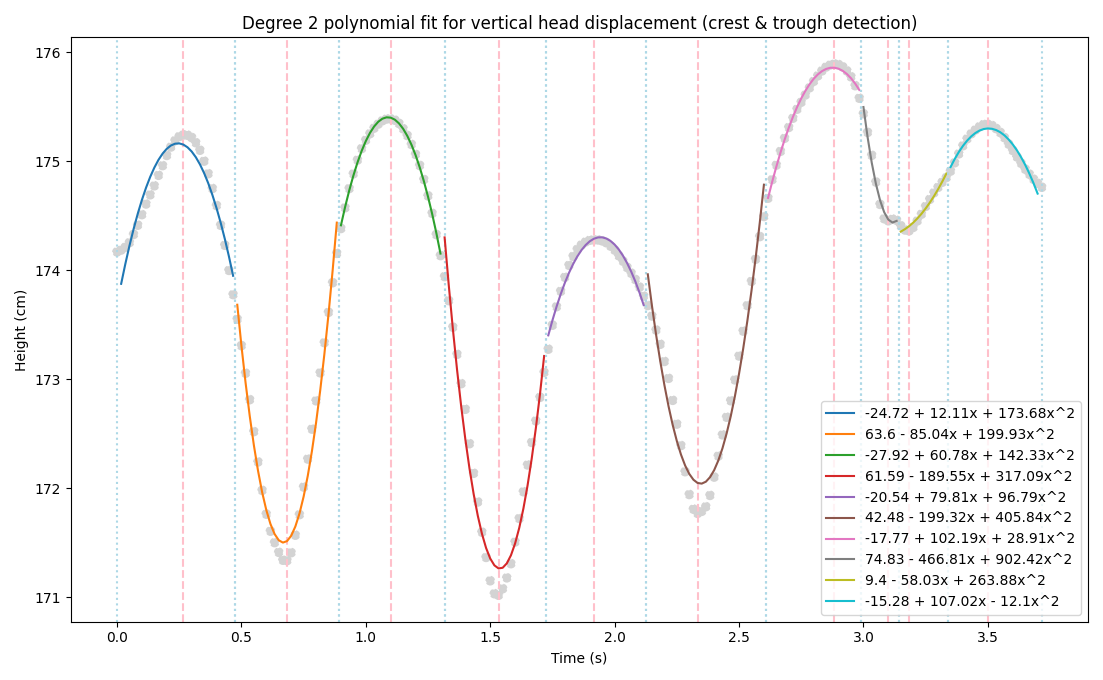
\includegraphics[width=\textwidth]{p_peaks_head_2.png}
    \caption{Quadratic fitting for vertical head oscillation data with crest \& trough detection} 
    \label{peaks_head}
\end{figure}

Figure \ref{peaks_head} demonstrates this detection method in action - the red
dashed vertical lines show the point at which a crest or trough was detected,
and the blue dotted lines show the start \& end of each fitting region, these
are placed between each creast or trough. Compared to the naive fit seen in
Figure \ref{naive_head}, this is certainly a much better outcome.

\begin{figure}[H]
    \centering
    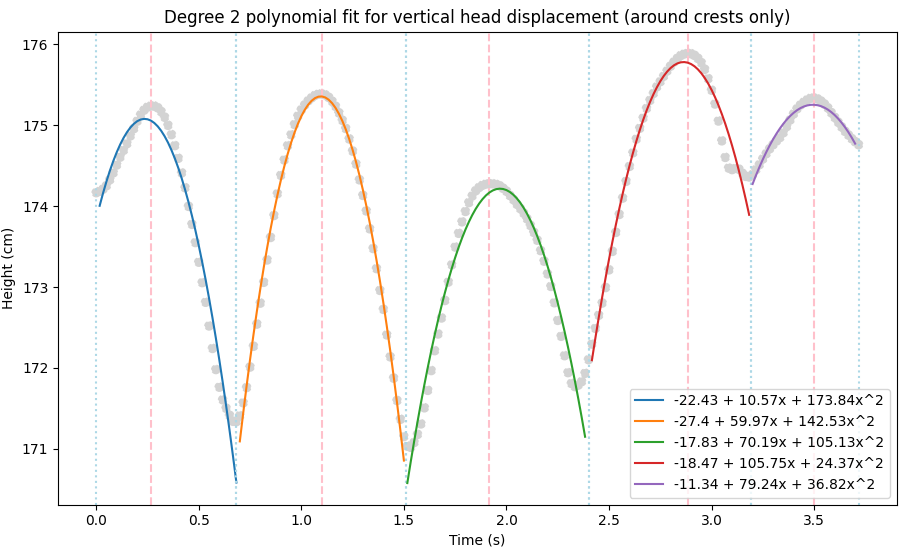
\includegraphics[width=\textwidth]{p_peaks_crestsonly_head_2.png}
    \caption{Quadratic fitting for vertical head oscillation data with crest detection only} 
    \label{crestsonly_head}
\end{figure}

The sharpness of the troughs seen in the head movement data poses an interesting
question - how would the accuracy of the model vary if only the crests were used
as the bases around which the quadratic are to be fit? Figure
\ref{crestsonly_head} illustrates one such example, and interestingly, it seems
that even with this, virtually no important information appears to be lost, yet
the number of equations has been reduced to half, all of which are, naturally,
concave down.

\begin{figure}[H]
    \centering
    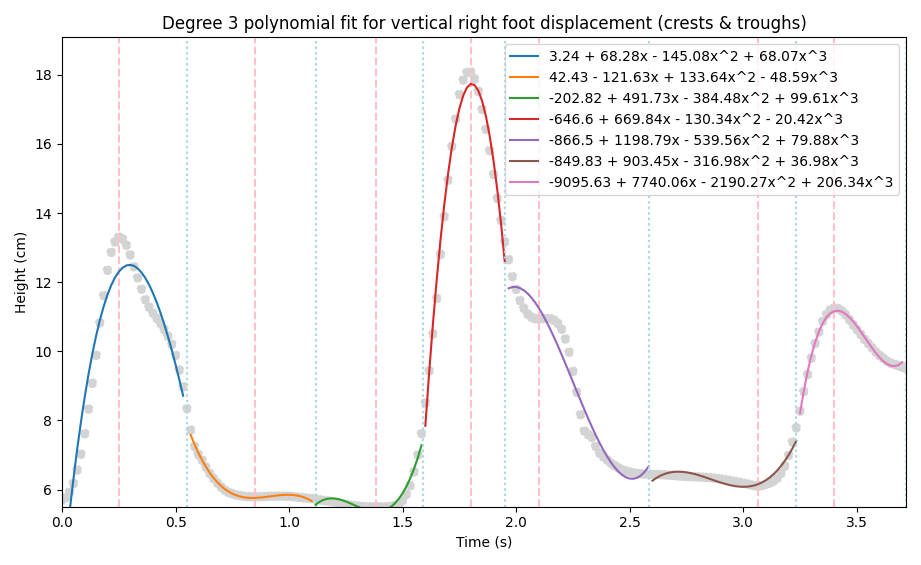
\includegraphics[width=\textwidth]{p_peaks_right_3.png}
    \caption{Cubic fitting for vertical right foot oscillation data with crest \& trough detection} 
    \label{peaks_right}
\end{figure}

% In order to better model the vertical oscillation while walking in general, it
% may be more worthwhile trying to model each individual crest and trough.

\end{document}